% Created 2016-06-11 Sat 09:14
\documentclass[9pt,b5paper]{article}
\usepackage{fontspec}
\usepackage{graphicx}
\usepackage{xcolor}
\usepackage{xeCJK}
\setCJKmainfont{Songti SC}
\usepackage{longtable}
\usepackage{float}
\usepackage{textcomp}
\usepackage{geometry}
\geometry{left=0.1cm,right=0.1cm,top=0.1cm,bottom=0.1cm}
\usepackage{multirow}
\usepackage{multicol}
\usepackage{algorithm}
\usepackage{algorithmic}
\usepackage{latexsym}
\usepackage{natbib}
\usepackage{listings}
\usepackage{minted}
\usepackage[xetex,colorlinks=true,CJKbookmarks=true,linkcolor=blue,urlcolor=blue,menucolor=blue]{hyperref}
\author{deepwaterooo}
\date{\today}
\title{Programming Language Theory -- Summer 2016}
\hypersetup{
  pdfkeywords={},
  pdfsubject={},
  pdfcreator={Emacs 24.5.1 (Org mode 8.2.7c)}}
\begin{document}

\maketitle
\tableofcontents


\section{Introduction}
\label{sec-1}
\begin{itemize}
\item hw2: haskell practice exercise code for any practice due on 6/15/2016 11:55pm.
\item 
\item 
\item 
\item 
\item Considering that I understand the way how to traverse and draw different parts of the zombie, I know I could but don't have to take all the effort to draw all the fingers in order to make a "fighting" pose (a hand cube stands for another "zombie"-like rotatation for 2 or 3 different finger parts).
\item I don't like the latter part of the project during to rotating simply around the center, though I want to make the zombie walk (but I don't have enough time to work on it). While I will try to work on the walking for a few (3-4) hours tonight to be able to at least have some taste.
\item My team buddy's spiderman Dancing stage could simply be rendered by defining the four glVertex3d vertex ([-25, -9.4, 25], [25, -9.4, 25], [25, -9.4, -25], [-25, -9.4, -25]), tex coordinate four points (00 10 11 01), and a Texture. By including norm data, it supposed to have some lights.
\item Todos: 
\begin{itemize}
\item Speed a few hours (3-4) tonight to work on the zombie walking.
\item Need try hard to figure out animation, how to dance with time changes, or need to move according to keytype inputs triggers.
\item Sub obj\% for cubes, and spheres if I need and want to implement any sphere for head, or eyes. But it seems I won't have enough time for this one now. Will try these ones through other projects later on then.
\end{itemize}
\item A current rotatable zombie and my team buddy's spiderman are looking like:
\end{itemize}

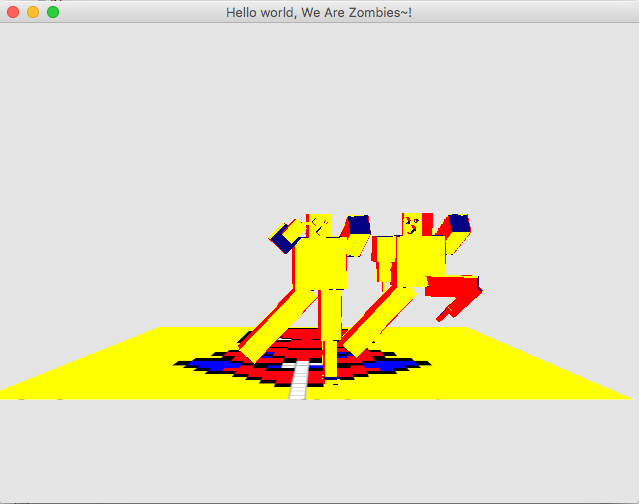
\includegraphics[width=.9\linewidth]{./pic/Screen_Shot_2016-05-31_at_1_52_26_AM.png}

\section{References}
\label{sec-2}
\subsection{Haskell}
\label{sec-2-1}
\begin{itemize}
\item Haskell \url{http://fleurer-lee.com/lyah/ready-begin.htm}
\item \url{http://wiki.jikexueyuan.com/project/haskell-guide/ready-go.html}
\item real world \url{http://rwh.readthedocs.io/en/latest/index.html}
\item \url{http://wiki.bitbegin.com/read/docs/9-haskell/1-haskell-brief-introduction}
\item \url{http://www.cnblogs.com/youxin/category/511831.html}
\item \url{https://wiki.haskell.org/OpenGL}
\item opengl \url{https://github.com/madjestic/Haskell-OpenGL-Tutorial}
\item \url{http://www.arcadianvisions.com/blog/2011/modern-opengl-with-haskell.html}
\item cube \url{https://github.com/haskell-opengl/GLUT/blob/master/examples/RedBook4/Cube.hs}
\item \url{https://wiki.haskell.org/OpenGLTutorial2}
\item 3d旋转魔方 \url{http://wenku.baidu.com/view/6e7b0d22915f804d2b16c1c1.html}
\item 
\item 
\end{itemize}

\subsection{opengl sgl}
\label{sec-2-2}
\begin{itemize}
\item rect hello world \url{https://lists.racket-lang.org/users/archive/2010-October/042474.html}
\item cube base: \url{https://gist.github.com/tonyg/5425736}
\item Texture Atlases \url{http://jeapostrophe.github.io/2013-05-06-texture--post.html}
\item Planet Cute \url{http://docs.racket-lang.org/teachpack/2htdpPlanet_Cute_Images.html}
\item Texture \url{https://www.mail-archive.com/racket-users@googlegroups.com/msg03203.html}
\item \url{http://lists.racket-lang.org/users/archive/2010-November/043118.html}
\item sgl \url{https://github.com/racket/sgl}
\item cube \url{https://rosettacode.org/wiki/Draw_a_cuboid#Racket}
\item pict3d \url{https://github.com/ntoronto/pict3d}
\item pict3d \url{https://docs.racket-lang.org/pict3d/index.html}
\item buffering \url{https://lists.racket-lang.org/users/archive/2015-March/066355.html}
\item c++ racket ex \url{http://home.adelphi.edu/sbloch/class/archive/333/fall2013/examples/pentagon/}
\item \url{https://rosettacode.org/wiki/OpenGL#Racket}
\item 原理: \url{http://cuiqingcai.com/1867.html}
\item \url{http://cuiqingcai.com/1867.html}
\item 2d \url{http://cuiqingcai.com/1597.html}
\item tech cube \url{http://wiki.jikexueyuan.com/project/opengl-es-basics/3d-images.html}
\item colorful \url{http://cs317y982s961535.blogspot.com/2010/04/2-3d.html}
\item \url{http://www.d3dweb.com/Documents/201202/15-15182458704.html}
\item define-struct \url{http://lists.racket-lang.org/users/archive/2008-July/026133.html}
\item class ex \url{https://learnxinyminutes.com/docs/racket/}
\item gui \url{https://docs.racket-lang.org/pict3d/rendering.html}
\end{itemize}
\subsection{Animation}
\label{sec-2-3}
\begin{itemize}
\item 3d programming: \url{http://cs317y982s950831.blogspot.com/}
\item ruby \url{https://www.youtube.com/watch?v=Iq5YbRDYVE4}
\item ex \url{https://www.ntu.edu.sg/home/ehchua/programming/opengl/CG_Examples.html}
\item sphere Texture \url{http://www.angelfire.com/linux/nexusone/projects.html}
\item sphere \url{https://www.opengl.org/discussion_boards/showthread.php/137753-Texture-map-on-a-gluSphere}
\item s trs \url{https://www.opengl.org/discussion_boards/showthread.php/163561-How-to-posistion-a-gluSphere}
\item emacs lambda \url{http://ergoemacs.org/emacs/emacs_pretty_lambda.html}
\item ani example \url{https://groups.google.com/forum/#!topic/racket-users/ZQ_6_cIirDk}
\end{itemize}
\subsection{Texture}
\label{sec-2-4}
\begin{itemize}
\item \url{https://gist.github.com/tonyg/5425736}
\item \url{http://stackoverflow.com/questions/30709454/racket-opengl-glviewport-not-correctly-mapping-normal-coordinates-to-window-coo}
\item \url{http://lists.racket-lang.org/users/archive/2010-November/043118.html}
\item main \url{https://gist.github.com/tonyg/5425736}
\end{itemize}

\subsection{OOP}
\label{sec-2-5}
\begin{itemize}
\item oop \url{https://docs.racket-lang.org/guide/classes.html}
\item creating classes \url{https://docs.racket-lang.org/reference/createclass.html}
\item struct-copy \url{http://yuyang0.github.io/notes/scheme.html}
\end{itemize}

\subsection{robot dance}
\label{sec-2-6}
\begin{itemize}
\item \url{https://www.youtube.com/watch?v=lacAgc7rv1o}
\item \url{https://www.youtube.com/watch?v=AoCXPicEa8o}
\item \url{https://www.youtube.com/watch?v=wQ4KXoFHwL4}
\end{itemize}

\subsection{other}
\label{sec-2-7}
\begin{itemize}
\item framework \url{https://github.com/NetEase/lively-logic}
\item \url{https://www.youtube.com/watch?v=SCh0zmP6R5A}
\item \url{https://www.youtube.com/watch?v=ayqhX9UA6FY}
\item \url{http://racket.tchen.me/practical-racket.html}
\item 图形:\url{https://www.zhihu.com/question/20789155}
\item threads \url{http://www.ithao123.cn/content-4141200.html}
\item \url{http://docs.racket-lang.org/guide/classes.html}
\item \url{https://docs.racket-lang.org/quick/}
\item \url{http://docs.racket-lang.org/draw/index.html}
\end{itemize}
% Emacs 24.5.1 (Org mode 8.2.7c)
\end{document}